\section{Remote Vision Virtual Subsystem}%
\label{sec:remote-visi-subsyst-design}
The \glsfirst{rvvs} is mainly responsible for providing visual feedback to the
user of the vehicle's surroundings to assist its navigation. Additionally, it should offload the
\gls{nvs} from other intensive, but no so critical, tasks --- like
telemetry data --- as well as provide redundant paths for communications,
especially in the most critical conditions, like off-grid navigation with the
inclusion of the \gls{gprs} module. Thus, as aforementioned and illustrated in
Fig.~\ref{fig:initial-design-2}, it interfaces three different subsystems:
\gls{nvs} via RS232 communication; smartphone via Wi-Fi or \gls{gprs}; and the
web camera.

The \acrshort{rvvs} design was divided into three phases, corresponding to the
functional, object and dynamic models.
%
\subsection{Functional model}%
\label{sec:functional-model-rvvs}
The functional model describes the functionalities of the system from the
actors' perspective, illustrated in Fig.~\ref{fig:rvvs-use-cases-diag} by an use
case diagram. Two actors were identified: \gls{nvs} and Smartphone. The
Smartphone acts a proxy for user interaction, thus for clarity purposes, the
actor was named \emph{User}. Three main set of features were identified, namely:
\begin{enumerate}
\item \textbf{Communication}: deals with the communications interfaces between the
  various subsystems, further decomposed into the required functionalities for
  each interface (\emph{Comm Functions}). The \emph{User} may communicate with
  the \gls{rvvs} subsystem via GPRS or Wi-Fi, thus requiring the latter to
  provide network discovery capabilities, alongside with the conventional
  connect, send, receive and  disconnect functionalities. Additionally, it may
  also required periodic \textit{KEEP ALIVE} pings to check if the connection is
  still on. The \acrshort{nvs} communicates via RS232, which does not require
  network discovery. Lastly, the user may require sensor information, which
  could potentially be connected to the \gls{rvvs} subsystem (e.g., in a
  \gls{i2c} network) for offloading the \gls{nvs} subsystem.
\item \textbf{Image Acquisition}: responsible for providing visual feedback
  to the user. It can be configured, started, stopped and captured.
\item \textbf{Processing}: responsible for processing: user commands for image
  acquisition or forwarding them to the \gls{nvs} subsystem as a redundant path;
  telemetry data, such as, overall distance traversed, maximum speed so far,
  and operation time.
\end{enumerate}
% Use case diagrams
\begin{figure}[!hbt]
\centering
    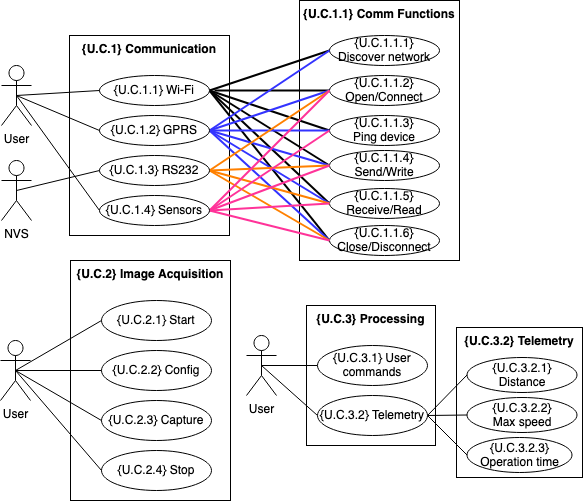
\includegraphics[width=0.5\textwidth]{./img/rvvs-use-cases-diag.png}
  \caption{Use case for \acrshort{rvvs} subsystem}%
\label{fig:rvvs-use-cases-diag}
\end{figure}
% Dynamic model
\subsection{Dynamic model}%
\label{sec:dynamic-model-rvvs}
The dynamic model describes the internal behaviour of the system, represented in
\gls{uml} by sequence, state-machine, and activity diagrams.

The sequence
diagram represents the sequence of events related to a particular use
case. It aids to refine use cases and identify software objects (entity,
boundary, control), providing a well-established path for the implementation of
system's functionalities.

On the other hand, state-machine diagrams provide an overview of the system
functionalities and how they interact, i.e., the system's states, transitions,
and response to stimulus, internal or external. This makes it an excellent tool
for designing overall system behaviour. Fig.~\ref{fig:state-mach-diag-legend}
identifies the main elements used in the state-machine diagram.

The state-machine diagram for the \gls{rvvs} subsystem is depicted in
Fig.~\ref{fig:rvvs-sync-state-diag}. On system startup is performed an
initialization procedure, loading user-defined and machine settings and
initializing the required hardware. After initialization is completed, four main
processing units are executed in parallel until system is shutdown, namely:
\begin{itemize}
\item \textbf{Wi-Fi Manager}: manages Wi-Fi connection;
\item \textbf{RS232 Manager}: manages RS232 connection;
\item \textbf{Main}: idle processing unit; parses messages received through the
  available communications channels and, if a
  command is detected, pushes it to a command queue for later execution.
\item \textbf{Scheduler}: periodically executed processing unit, responsible for
  executing periodical tasks and spawning tasks as a response to issued
  commands, with different priority levels.
  \begin{itemize}
  \item \textbf{Task}: spawned as a response to a command, performs the
    required associated function and has a low expected lifetime. The commands
    can be classified as user, \gls{nvs}, telemetry data, image acquisition, or
    communications.
  \end{itemize}
\end{itemize}

Lastly, an example of a more refined state-machine diagram, in this case for
communications, is illustrated in Fig.~\ref{fig:rvvs-comm-state-diag}. In the
initial state, a connection request is expected and if accepted, authentication
is requested. If successfully authenticated, the Communication Manager is ready
to communicate, handling incoming/outgoing data by notifying the relevant
entities and performing the associated operations. The RS232 does not require
connection and authentication management, thus yielding only the states
\texttt{readyToCommunicate}, \texttt{MsgReceived}, and \texttt{MsgToSend}. 
% State-machine diagram legend
\begin{figure}[!hbt]
\centering
    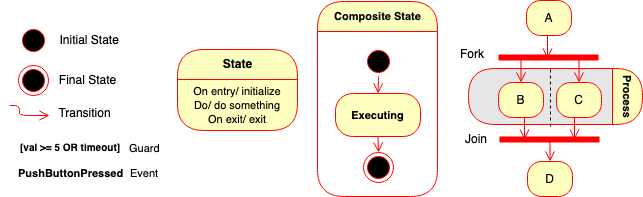
\includegraphics[width=0.7\textwidth]{./img/state-diag-caption.png}
  \caption{State-machine diagram}%
\label{fig:state-mach-diag-legend}
\end{figure}
% State-machine diagram for Synchronization
\begin{figure}[!hbt]
\centering
    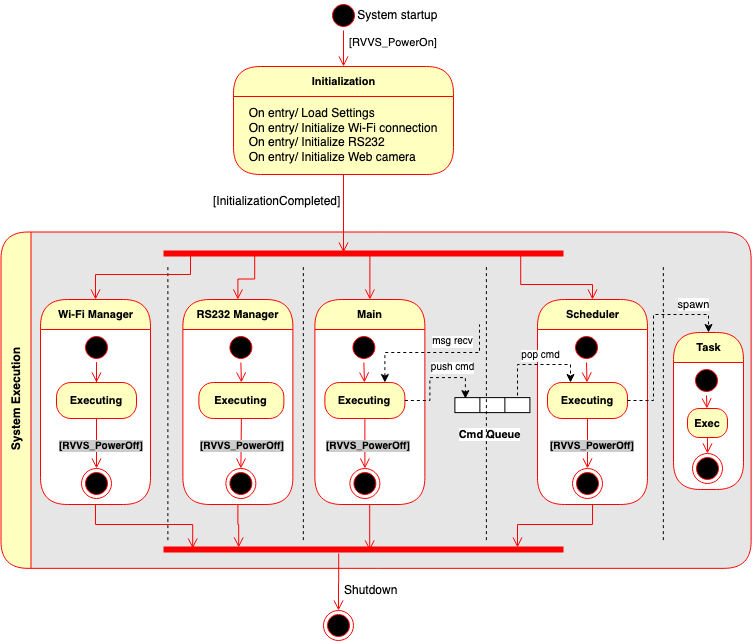
\includegraphics[width=0.8\textwidth]{./img/rvvs-sync-state-diag.png}
  \caption{\acrshort{rvvs} state-machine diagram}%
\label{fig:rvvs-sync-state-diag}
\end{figure}
% State-machine diagram for Communication
\begin{figure}[!hbt]
\centering
    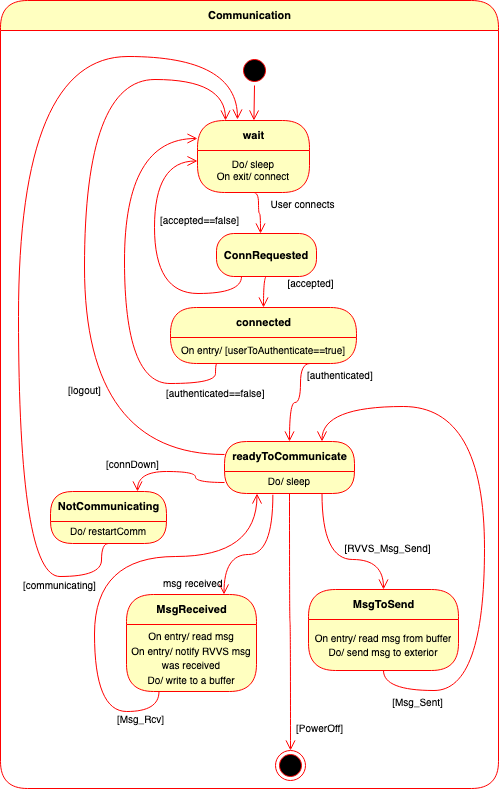
\includegraphics[width=0.5\textwidth]{./img/rvvs-comm-state-diag.png}
  \caption{Communication state-machine diagram}%
\label{fig:rvvs-comm-state-diag}
\end{figure}
%
\subsection{Subsystem decomposition}%
\label{sec:subsyst-decomposition-rvvs}
Following the same design rationale indicated in
Section~\ref{sec:navigation-system-design} for the \gls{nvs} subsystem, the
the \gls{rvvs} system should be decomposed into smaller, more tractable,
subsystems for easier development. Furthermore, modularity and reuse, whenever
is possible, should be key design guidelines.

The subsystem decomposition for
\gls{rvvs} is illustrated in Fig.~\ref{fig:rvvs-comm-state-diag}, taking into
account these considerations. Thus, \texttt{OS}, \texttt{COM Transport}, and
\texttt{COM Data} packages are reused from \gls{nvs} for the following reasons:
\gls{rvvs} requires concurrent/parallel processing as provided by the
\texttt{OS} package in a thread-safe way; it shares the communication interface
with \gls{nvs} (RS232), as provided by the \texttt{COM} packages. The same idea
is extensible to the Wireless Communication (\texttt{WCOM} package), with the
transport layer comprised of a \texttt{Manager}, a \texttt{RedundancyEngine} and
a \texttt{Stream} for packet serialization/deserialization, and a low-level
layer dependent of the technology used (Wi-Fi/GPRS). For \texttt{Image
  Acquisition}, a \texttt{Manager} handles image acquisition functionalities,
with the \texttt{Frame} acting as image data container; low-level layer
\texttt{Img::LL} handles the hardware interface and low-level
details. Completing the system stack is the \texttt{Telemetry} package,
responsible for managing the telemetry data as required. This package could have
a direct interface with the sensors, but, for the time being, it tracks
information received by the \gls{nvs} subsystem.

At the top of the software stack is the actual software executed on top of the
system stack, containing the application logic and management. Thus, the
\texttt{App::Manager} package is a event-driven processing unit, listening for
relevant events signalled by the layers below and handling those events, as the
one generated by successfully parsing of commands arriving from the available
communications channels. 
% Full stack overview for RVVS
\begin{figure}[!hbt]
\centering
    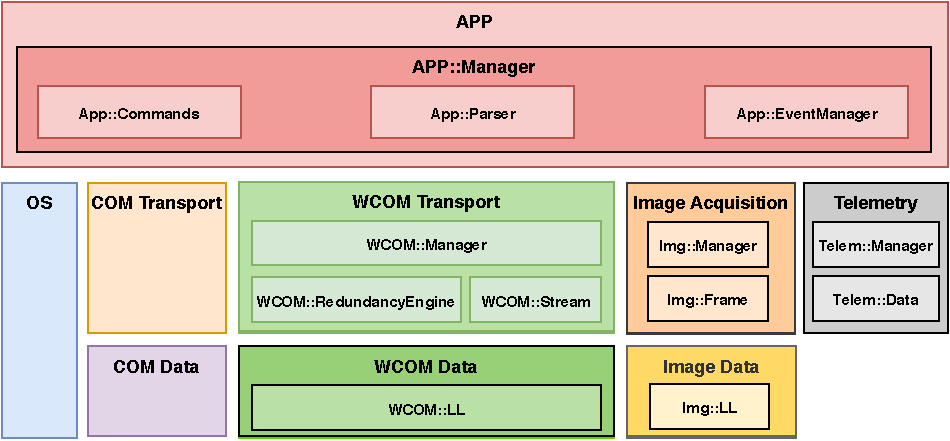
\includegraphics[width=0.8\textwidth]{./img/rvvs-full-stack.pdf}
  \caption{\acrshort{rvvs} full stack overview}%
\label{fig:rvvs-full-stack}
\end{figure}
%
\subsection{Object model}%
\label{sec:object-model-rvvs}
The object model, represented in \gls{uml} with class diagrams, describes the
structure of the system in terms of objects, attributes, associations, and
operations. 
%


%%% Local Variables:
%%% mode: latex
%%% TeX-master: "../../../dissertation"
%%% End:
